
\chapter{Hyperelliptic curves and curves of genus 2 and 3}
\label{genus 2 and 3 chapter}

\section{Hyperelliptic curves}
\label{hyperelliptic}

Recall that a hyperelliptic curve $C$ is a curve of genus $\geq 2$
admitting a map $\pi : C \to \PP^1` `$ of degree 2.
We met hyperelliptic curves in Chapter~\ref{RiemannRochChapter} and proved
that
\index{hyperelliptic curve}%
the canonical
map from $C$ is the composition of $\pi$ with
the embedding of $\PP^1$ in $\PP^{g-1}$ as a rational normal curve,
showing in particular that $\pi$ is unique up to automorphisms of $\PP^1$.

 We used this to show that every special
linear series on a hyperelliptic curve is a sum of a multiple of  the
unique $g^1_2$ plus basepoints. We will begin this chapter with an
explicit construction of hyperelliptic curves and use it to give a
concrete computation of the canonical series, reproving what we did in
Chapter~\ref{RiemannRochChapter}.
Then we will consider the projective embeddings of curves of
genus 2 (which are all hyperelliptic) and genus 3.

There will be a further discussion of hyperelliptic curves in
Chapter~\ref{ScrollsChapter}.

\subsection*{The equation of a hyperelliptic curve}

 Because the degree of the canonical map is  2, each point in $\PP^1$
has either two distinct preimages, or only one; in the latter case,
this point is a
ramification point
\index{ramification!point}%
with ramification index 1; that is, the
map is given in terms of local analytic coordinates on $C$ and $\PP^1$
by $z \mapsto z^2` `$. In particular, both the
ramification divisor
\index{ramification!divisor}%
and
the
branch divisor
\index{branch divisor}%
(as defined in Chapter~\ref{RiemannRochChapter}) are
reduced. By
Hurwitz's formula
\index{Hurwitz's theorem}%
there are exactly $2g+2$ branch points
in $\PP^1` `$. These points determine the curve:

\begin{theorem}
\label{hyperelliptic existence}
There is a unique smooth projective hyperelliptic curve $C$ expressible
\index{hyperelliptic curve!determined by $2g+2$ points}%
as a
$2$-sheeted cover
\index{2-sheeted cover!of $\PP^1$}%
of $\PP^1$ branched over any given set of $2g+2$
distinct points $\{q_{1}, \dots, q_{2g+2}\}$.
\unif
\end{theorem}

\begin{proof}
We
will exhibit
 such a curve,
leaving the proof of uniqueness to Section~\ref{branched covers}.
If the coordinate of the point $q_i \in \PP^1$ is $\lambda_i$,
we take for $C$
the smooth
projective model
\label{projective model}%
of the affine curve
  $$
 \tsty\let\big\Big
C^\circ = \big\{@(x,y) \in \AA^2 \bigm|  y^2 = \prod\limits_{i=1}^{2g+2}
(x - \lambda_i)@\big\}.
$$
Note that we're choosing a coordinate $x$ on $\PP^1$ with the point
$x = \infty$ at infinity not among the $q_i$, so that the preimage of
$\infty \in \PP^1$ is two points $r, s \in C$. Concretely, we see that
as $x \to \infty$, the ratio $y^2/x^{2g+2}$
approaches
$1$, so that
$$
\lim_{x \to \infty} @ \frac{y}{x^{g+1}}  =  \pm 1.
$$
  The two possible values of this limit correspond to the two points
  $r,s \in C$.
\end{proof}

The curve $C$
thus constructed
is \emph{not} simply the closure of the affine curve
$C^\circ \subset \AA^2$ in either $\PP^2$ or $\PP^1 \times \PP^1` `$: as
you can see from a direct examination of the equation, each of these
closures will be singular at the (unique) point at infinity.

To give a smooth projective model of
a
hyperelliptic curve $C$ with
given branch divisor, we divide the $2g+2$ branch points  into two sets
of the
same size,
 $\{q_1,\dots,q_{g+1}\}$ and $\{q_{g+2}, \dots,
q_{2g+2}\}$. We can then take $C$ to be the closure in $\PP^1 \times \PP^1$
of the  locus
  $$
 \tsty\let\big\Big
  \big\{@(x,y) \in \AA^2  \bigm|  y^2\prod\limits_{i=1}^{g+1} (x - \lambda_i)
  = \prod\limits_{i=g+2}^{2g+2} (x - \lambda_i)@\big\};
  $$
  in projective coordinates, this is
   $$
 \tsty\let\big\Big
  C  =  \big\{@((X_{0},X_{1}), (Y_{0},Y_{1})) \in \PP^1 \times
  \PP^1  \bigm|  Y_1^2\prod\limits_{i=1}^{g+1} (X_1 - \lambda_iX_0) =
  Y_0^2\prod\limits_{i=g+2}^{2g+2} (X_1 - \lambda_iX_0)@\big\}.
  $$
To see that $C \subset \PP^1 \times \PP^1$ is smooth we note that it is a
curve of
bidegree
\index{bidegree}%
$(2,g@{+}@1)$ in $\PP^1 \times \PP^1` `$, and the formula for
the genus of a curve in $\PP^1 \times \PP^1$ derived in
Example~\ref{Div of quadric} tells us that such a curve has
arithmetic genus $g$, and thus no singular points.

From this model, we deduce:

\begin{corollary}
\label{relation on ramification points}
If $C$ is a hyperelliptic curve  and $p_1,\dots,p_{2g+2} \in C$ are the
ramification points of the unique degree $2$ map $C \to \PP^1` `$, then for any
division of $\{1,\dots,2g+2\}$ into two sets $A,B$ of cardinality $g+1$,
$$
\sum_{i\in A} p_{i}   \sim  \sum_{i\in B}p_{i}.
$$
\end{corollary}

\begin{proof}
The abstract curve $C\subset \PP^{1}\times \PP^{1}$ above
is independent of the
choice of $A$ and $B$,
since in any case the projection to the
first factor
is ramified at the same set $p_{1}, \dots, p_{2g+2}$. Given the
representation above, the sets
$\{p_i\mid i\in A\}$ and  $\{p_i\mid i\in B\}$
are
preimages of $(0,1)$ and
$(1,0)$ in the second factor.
\end{proof}

 The map $\iota : C \to C$ that exchanges the two points in each reduced
 fiber of the map $C \to \PP^1$ and fixes the ramification points is
 algebraic: in terms of the last representation of $C$, it is given by
 $((X_0,X_1), (Y_0,Y_1)) \mapsto  ((X_0,X_1), (Y_0,-Y_1)) $. The map
\index{involution, hyperelliptic}%
 $\iota$ is called the \emph{hyperelliptic involution} on $C$.

\subsection*{Differentials on a hyperelliptic curve}
%  \label{hyperelliptic differentials}

We can give a pleasantly concrete \null description of the differentials,
and thus the
canonical linear series,
\index{linear series!canonical}%
on a hyperelliptic curve $C$
by working with the affine model $C^\circ = V(f) \subset \AA^2` `$, where
$$
f(x,y) = y^2 - \prod_{i=1}^{2g+2} (x - \lambda_i).
$$
We will again denote the two points at infinity (that is, the two points
of $C \setminus C^\circ$) by $r$ and $s$; for convenience, we'll denote
the divisor $r+s$ by $D$. We write $\pi:C \to \PP^1$ for the morphism
that, on $C^\circ$, sends $(x,y) \in C$ to $x$.

We can construct a differential form on $C$ by following the proof of
Hurwitz's theorem
\index{Hurwitz's theorem}%
in
Chapter~\ref{RiemannRochChapter}.
Let $dx$ denote the usual differential on $\PP^1$ having a double
pole at infinity, and consider $\pi^*dx$ on $C$.  The function $x$ is
regular on $C^\circ$, and is a local parameter over points other than
the $\lambda_i$; from the local description of the map $\pi$, we see that
$\pi^*dx$ is regular on $C^\circ$  with simple zeros at the ramification
points $q_i = (\lambda_i, 0)$. Since $dx$ has a double pole at the
point at $\infty\in \PP^1$ and $\pi$ is a local isomorphism near $r$
and $s$, the differential $\pi^*dx$ has double poles at the points $r$
and $s$. Thus the canonical
divisor of $C$ is
$$
 K_C \sim (dx) \sim R - 2D,
$$
where $R$ denotes the ramification divisor, in this case the sum of the
ramification points.

How can we find differentials that are regular everywhere on $C$? If we
divide $dx$ by $x^2$ (or any quadratic polynomial in $x$) to kill the
poles we  introduce new poles in the finite part $C^\circ$ of $C$.

Instead, we want to multiply $dx$ by a rational function with zeros
at $r$ and $s$, but whose poles occur only at the points where $dx$
has zeroes\emdash that is, the points $\lambda_i$.  A natural choice is the
reciprocal of the partial derivative $f_y \colonequals  \partial f/ \partial y =
2y$, which vanishes at the points $q_i$, and has  a pole of order $g+1$
at each of the points $r$ and $s$ (reason: $y/x^{g+1}$ approaches $\pm
1$ as $x$ goes to infinity, and $x$ has a pole of order 1 at $\infty\in
\PP^{1}$ and thus also at each of $r,s$). In other words, as long as $g
\geq 1$, the differential
$$
\omega = \pi^*\left(\frac{dx}{f_y}\right)
$$
is regular, with divisor
$$
(\omega) = (g-1)@r + (g-1)@s = (g-1)@D.
$$
The remaining regular differentials on $C$ are now easy to find: Since
$x$ has only a simple pole
at the two points at infinity we can  multiply $\omega$ by any $x^k$ with
$k = 0, 1, \dots, g-1$.
This gives us $g$ differentials
$$
\omega, x\omega, \dots, x^{g-1}\omega
$$
that are independent, and so form a basis for $H^0(K_C)$.

With this description of the differentials, we can see clearly why the
canonical map of a hyperelliptic curves is degree 2 onto a rational
normal curve, as proved in Chapter~\ref{RiemannRochChapter}:
the relations on
$
\omega, x\omega, \dots, x^{g-1}\omega
$
are the relations on $x^i` `$, and we see that the canonical image is the
rational normal curve
\index{rational!normal curve}%
 of degree $g-1$.

\section{Branched covers with specified branching}
\label{branched covers}

Given a curve $B$ and points
$\thinmuskip=3mu plus 2mu p_1,\dots,p_b$ in $B$,
what are the branched covers $\pi :\nobreak C \to\nobreak B$
of degree $d$ with specified branching over each of the points $p_i$,
up to isomorphism over $B$?
We will reduce this question to the classification of topological
covering spaces of the complement $U = B \setminus \Delta$; we will
then use properties of the fundamental group of $U$ to enumerate such
covering spaces. We will prove the uniqueness of hyperelliptic curves with specified branch points
at the end of this section as a special case of a general analysis of branched covers.

\begin{theorem}
 Let $B$ be a smooth curve, let $\Delta\subset B$ be a finite set of
 points, and let $U \colonequals  B\setminus \Delta$.
If $\pi^\circ : V \to U$ is a topological covering space then $V$ may
be given the structure of a
Riemann surface
\index{Riemann surface}%
in a unique way so that
the map $\pi^\circ$ is holomorphic; and $V$ may be compactified to a
compact Riemann surface $C$ in a unique way such that the map $\pi^\circ$
extends to a holomorphic map $\pi : C \to B$.
\unif
\end{theorem}

\begin{proof}
The space $V$ inherits the structure of a complex manifold from $U$
because if $D \subset U$ is any simply connected coordinate chart,
then the preimage $({\pi^\circ})^{-1}(D)$ is a disjoint union of $d$
copies of $D$, and we may use them as coordinate charts on $V` `$.

To compactify $V$ we observe that if $D^* = \{ z \in \CC \mid 0 < |z|
< 1 \}$ is a punctured disc, then
the map
$z \mapsto z^n$ on the unit disk
restricts to a connected $n$-fold covering
space $D^*\to D^*` `$.
Since $\pi_1(D^*) = \ZZ$, any connected covering space $E$ of degree $n$
is homeomorphic to this one
by a homeomorphism inducing the identity on the target of $\pi$.
If we  define a holomorphic structure on $E$ by pulling back the one on
$D$, then
this homeomorphism is biholomorphic.

Thus if $D_i$ is a small neighborhood of the point $p_i \in B$
biholomorphic to a disc, then the preimage  in $V$ of the punctured
disc $D_i^* \colonequals  D_i \cap U$ is a disjoint union of punctured discs
$E_{i,j}^{*}$. The maps $E^{*}_{i,j} \to D_{i}^{*}$
are homeomorphic to the maps $z\mapsto z^{n_{i,j}}$
of the punctured unit disc
for some
$n_{i,j}$. Because of the way the holomorphic structure
of $V$ is defined, the maps
$E^{*}_{i,j} \to D_{i}^{*}$
are actually
holomorphic. Thus they extend holomorphically
to maps of the full disks $E_{i,j}\to D_{i}$ and $V@\cup@ \bigcup` E_{i,j}$
is a compact Riemann surface in a unique way.
\end{proof}

The problem of classifying smooth curves $C$ that have a map $\pi : C \to B$
of~degree $d$ thus becomes one of classifying covering spaces of $U$.
\index{covering space}%

\subsection*{Branched covers of $\PP^1$}

We continue with the notation $U = B\setminus \Delta$, now supposing
\index{branched cover of $\PP\sp1$}%
that $B = \PP^1_\CC$, the Riemann sphere. Again, let $\pi:V\to U$ be a
covering space.

Choose a basepoint $p_0 \in U$, and draw simple, nonintersecting arcs
$\gamma_i$ joining $p_0$ to $p_i$ in $U$. If $\Sigma$ is the complement
of the union of these arcs in the sphere, then the preimage of $\Sigma$
in $V$ will be the disjoint union of $d$ copies of~$\Sigma$, called the
\index{sheet|defi}%
\emph{sheets} of the cover; label these $\Sigma_1,\dots,\Sigma_d$.

Given $U$, elementary homotopy theory asserts the existence of a bijection
between coverings $V \to U$ of $U$ of degree $d$ (up to homeomorphisms
of $V$ fixing~$U$) and group
homomorphisms
   $$
 M:  \pi_1(U, p_0) \to S_d,
   $$
to the symmetric group on $d$ letters, up to inner automorphisms of
\index{symmetric group}%
\index{inner automorphism}%
$S_{d}$. The map $M$ is called the \emph{monodromy} of the covering:
given $V \to U$
and a labeling of the $d$ sheets of $V$ over the point
$p_0$, the value of $M$ at a loop  $\beta$ in $U$ based at $p_0$
is the
permutation of the points of $\pi^{-1}(p_0)$ given by sending a point
$q \in \pi^{-1}(p_0)$ to the endpoint of the unique lift of $\beta$
starting at $q$. A permutation $\sigma$ of the labels  of the sheets
leads to a map $M'$ equal to the composition of $M$ with conjugation
by $\sigma$.

A convenient set of generators of $ \pi_1(U, p_0)$ is the set of paths
$\beta_i$ indicated in Figure~\ref{pi 1 generators}: starting at $p_0$,
going out along the arc $\gamma_i$ until just short of $p_i$, going
once around $p_i$ and then going back to $p_0$ along the same path
$\gamma_i$. The fundamental group
\index{fundamental group}%
\index{free group}%
 of $U$ is the free group generated
by the paths $\beta_1,\dots \beta_b$ \null modulo the relation $\prod_{i=1}^b
\beta_i = 1$
which comes from the fact that the sphere minus the part enclosed by
the paths $\beta_i$ is
contractible.
{\meshing\par}

\begin{figure}
\centerline{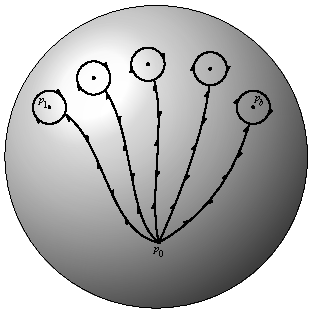
\includegraphics[height=1.8in]{main/Fig05-1}}
\vskip-6pt
 \caption{Generators for the fundamental group of a multiply punctured
 sphere.}
 \label{pi 1 generators}
\end{figure}

Given a degree $d$ covering space $V$ and a labeling of the $d$ sheets
over the point $p_0$, let $\tau_i$ be the permutation of $\{1,2,\dots,d\}$
corresponding to the path $\beta_i$. The space $V$ is connected if and
only if the $\tau_{i}$ generate a transitive subgroup of~$S_{d}$. The
case $d=2$ is illustrated in Figure~\ref{square root function graph}.

If we start from a map of Riemann surfaces $C\to \PP^{1}$ that is
 simply branched, and take $V$ to be the complement of the set of
 branch points,
 then each $\tau_i$ is a transposition.

\begin{figure}
\vskip1pt
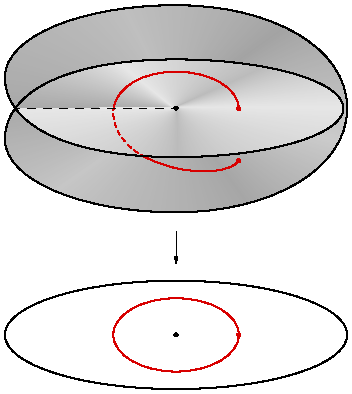
\includegraphics[height=2.1in,trim=0 2 0 0,clip]{main/Fig05-2-good}
\vskip-3pt
\caption{Local picture of a simple branch point $z \mapsto z^2` `$.
}
\index{simple branch point}%
\index{branch point!simple}%
\label{square root function graph}
\end{figure}

Summarizing we have proven:
   \begin{lemma}
   \label{branched cover classification}
   Let $p_1,\dots, p_b \in \PP^1$ be any $b$
distinct
points. There is a
   natural bijection between
   \begin{enumerate}
   \item the set of  simply branched covers $\pi : C \to \PP^1$ of
   degree $d$, branched over the points $p_i$, up to isomorphism over
   $\PP^1$; and
   \item the set of $b$-tuples of transpositions $\tau_1, \dots, \tau_b
   \in S_d$ such that
\smallbreak
\begin{enumerate}
 \item $\prod \tau_i$ is the identity, and
 \item $\tau_1, \dots,
   \tau_b$ generate a transitive subgroup of $S_d$,
\end{enumerate}
\smallbreak
\noindent modulo simultaneous
   conjugation by $S_d$.
   \qed
   \end{enumerate}
\let\qed\relax
   \end{lemma}

\begingroup \def\,{\kern1pt}
\begin{proof}[Proof \,of \,the \,uniqueness \,statement \,in
Theorem~\ref{hyperelliptic existence}.]
In the case of double covers of $\PP^1$ that is relevant to hyperelliptic curves, we note that
there is only one transposition in $S_2$. Thus there is a unique double
cover of $\PP^1$ with given branch points $p_1,\dots,p_b$. (The product
condition shows again that the number of branch points must be even.) This
completes the proof of Theorem~\ref{hyperelliptic existence}.
\emergencystretch1pt
\end{proof}
\endgroup

\begin{example}
In contrast to the situation of double covers of $\PP^1$, there are generally many
branched covers of specified degree  greater than 2 or with given branch points
and given conjugacy classes of the local monodromy.
The number of these is called
the \emph{Hurwitz number}
\index{Hurwitz number}%
of the configuration, and its computation in
general is the subject of a large and active literature; see for example
\cite{ELSV}.

To illustrate this, we can use Lemma~\ref{branched cover classification} to count the number of
degree 3 branched covers
\index{3-sheeted cover}%
$C \to \PP^1$ with given simple branch points, using that fact that every
odd permutation $\tau \in S_3$ is a transposition. Thus if $b$ is even
and  $\tau_1,\dots,\tau_{b-1} \in S_3$ are arbitrary transpositions,
then the product
$\tau_1\cdot \cdots\cdot \tau_{b-1}$ is also a
 transposition. It follows that the number of ordered $b$-tuples of
 transpositions $\tau_1,\dots,\tau_{b} \in S_3$ with $\prod \tau_i$
 equal to the identity is $3^{b-1}$. The requirement that the group
 generated by the $\tau_i$ is transitive eliminates just the three
 cases where all the $\tau_i$ are equal. The group $S_3$ acts on the
 set of $b$-tuples of permutations without stabilizing any $b$-tuple,
 so every cover corresponds to exactly 6 sequences
  $\tau_1,\dots,\tau_b$. In sum, the number of simply branched
  3-sheeted covers of $\PP^1$ with specified branch points
  $q_1,\dots,q_b \in \PP^1$ is
$$
\frac{3^{b-1} - 3}{6} \; = \; \frac{3^{b-2} - 1}{2}.
$$
One can use a similar strategy to count covers in other cases, when the
target has higher genus and/or the degree of the covering is larger,
but the combinatorics becomes more complicated.
\end{example}

\section{Curves of genus 2}
\label{genus 2 section}

Since  curves of genus 2 are hyperelliptic, everything we said above
applies to them; in particular, the canonical map $\phi_K : C \to \PP^1$
on a
curve of genus 2
\index{genus 2 curve!maps to $\PP\sp1$}%
 is the expression of $C$ as a double cover of
$\PP^1` `$, simply branched over 6 points in~$\PP^1` `$, which are unique up
to automorphisms of $\PP^1` `$.

In this section, we'll consider other maps from hyperelliptic curves $C$
to projective space, starting with maps $C \to \PP^1` `$.
See for example \cite{transcanonical} for a treatment of certain
embeddings of hyperelliptic curves of all genera.

\subsection*{Maps of $C$ to $\PP^1$}

The curve $C$ has a unique degree 2 morphism to $\PP^1$  associated
to the canonical system $|K_C|$. But there are many other morphisms to
$\PP^1` `$. For example, there is a 2-parameter
family of maps of degree 3:

 Let $\sL$ be an invertible sheaf of degree 3 on $C$. Since $3 > 2g-2$,
 the
Riemann--Roch theorem
\index{Riemann--Roch theorem}%
 tells us immediately that $h^0(\sL) = 2$, and
 there are two possibilities:

\begin{enumerate}
\item If the linear series $|\sL|$ has a basepoint $p \in C$,
then $h^0(\sL(-p)) = 2$, and hence $\sL$ must be of the form $\sL =
K_C(p)$. Conversely, if $\sL = K_C(p)$, then $h^0(\sL(-p)) = h^0(\sL)$, which
is to say $p$ is a basepoint of $|\sL|$. There is a 1-parameter family of
such $\sL$.

\item If $\sL$ is not of the form $\sL = K_C(p)$, then $|\sL|$ does not have
\label{genus 2 pencil} % used for page number
a basepoint, and so defines a degree 3 map $\phi_\sL : C \to \PP^1` `$.
\end{enumerate}

Since the variety $\Pic_3(C)$ has dimension $g= 2$ the general invertible
sheaf of degree 3 is of the second kind, and this gives a 2-parameter
family of such maps.

There are plenty of higher-degree maps as well: an invertible sheaf of
degree $d \geq 4 = 2g$ is basepoint free, and gives a map to $\PP^{d-2}$,
from which we can project in many ways
to $\PP^1` `$.

\subsection*{Maps of $C$ to $\PP^2$}
Next consider maps of a curve $C$ of genus 2 to the plane. By the Riemann--Roch
\index{genus 2 curve!maps to $\PP^2$}%
theorem, an invertible sheaf $\sL$ of degree 4 on $C$
has
$h^0(\sL)
= 3$ and is basepoint free by Corollary~\ref{degree 2g+1 embedding}, so
the linear series $|\sL|$  gives a morphism $\phi_\sL : C \to \PP^2` `$. The
invertible sheaf $\sL\otimes \omega_C^{-1}$ is either
$\omega_C$ or nonspecial; in either case, by the Riemann--Roch theorem,
it has at least one section,
so we may write $\sL\otimes \omega_C^{-1} = \sO_C(p+q)$ for some points
$p,q$. There are two possibilities:

\begin{enumerate}
\item If $p+q =  K_C$, then $\sL = \omega_C^2` `$. Since
the elements of $H^0(\omega_C)$ may be written as $\omega, x\omega$,
the map
$$
\Sym^2 H^0(\omega_C) \to H^0(\sL)
$$
 is injective, and since both sides are 3-dimensional vector spaces,
 they are equal. In other words, every divisor $D \sim 2K_C$ is the sum
 of two divisors $D_1, D_2 \in |K_C|$. We conclude that the map $\phi_\sL$
 is the composition of the canonical map $\phi_K : C \to \PP^1$ with the
Veronese embedding
\index{Veronese!map}%
 $\nu_2 : \PP^1 \to \PP^2$ of $\PP^1$ as a conic in
 the plane and the map $\phi_\sL$ is generically 2-to-1 onto the conic.

\item
\label{p+q not g12}
If $p+q \neq  K_C$  then $h^0(p+q) = 1$, so the pair $p,q$ is
unique. Furthermore,
 $h^0(\sL-p) = 2 =  h^0(\sL(-p-q))$ so
 $H^0(\sL(-p)) = H^0(\sL(-q))$ and $\phi_\sL(p) = \phi_\sL(q)$.
By the genus formula, the
$\delta$ invariant
\index{delta invariant@$\delta$ invariant}%
of this point must be 1. By
Exercise~\ref{delta=1 characterization}
 this is a
node
\index{node!on quartic}%
(if $p\neq q$) or
cusp
\index{cusp!on quartic}%
\index{quartic curve!with a node or cusp}%
(if $p=q$).
\end{enumerate}

Thus  for $\sL$ in an open subset of $\Pic_4(C)$ the image is a quartic
with a node; for a one-dimensional locus in $\Pic_4(C)$, the image is
a quartic with a cusp; and for one point in $\Pic_4(C)$ the image is
a conic.

\subsection*{Embeddings in $\PP^3$}

By Corollary~\ref{degree 2g+1 embedding} any invertible sheaf $\sL$ of
\index{genus 2 curve!embeddings in $\PP^3$}%
\index{quintic curve!of genus 2}%
degree 5 is very ample.
Write $\phi_\sL : C \to \PP^3$
for the map given by the complete linear
series $|\sL|$. Since $\phi_\sL$ is an embedding, we'll also denote the
image $\phi_\sL(C) \subset \PP^3$ by $C$ and write $\cO_C(1)$ for $\sL$.

What degree surfaces in $\PP^3$ contain the curve $C$? We start with
degree 2, and consider the restriction map
$$
H^0(\cO_{\PP^3}(2)) \to H^0(\cO_C(2)) = H^0(\sL^2).
$$
The space on the left has dimension 10; by the
Riemann--Roch theorem
\index{Riemann--Roch theorem}%
we have $h^0(\sL^2) = 2\cdot5 - 2 + 1 = 9$. It follows that $C$ lies
on a quadric surface $Q$. Since $C$ is not contained in a plane or a
union of planes, any quadric containing $C$ is irreducible; if there
were more than one such,
B\'ezout's theorem
\index{Bezout@B\'ezout's theorem}%
 would imply that $\deg C
\leq 4$. Thus $Q$ is unique.

We might ask at this point: is $Q$ smooth or a quadric cone? The answer
depends on the choice of invertible sheaf $\sL$.

\begin{proposition}
\label{genus 2 embedding}
Let $C \subset \PP^3$ be a smooth curve of degree $5$ and genus $2$, and
set $\sL = \sO_C(1)$. The unique quadric $Q$ containing $C$
  is singular if and only if
$$
\sL \cong K^2(p)
$$
for some point $p \in C$; in this case, the point $p$ maps to the vertex
of $Q$.
\end{proposition}

\begin{proof}

Suppose first that
$\sL \cong K^2(p)$ for some $p \in
C$. Then $\sL(-p) \cong K^2` `$, so that the map $\pi : C \to \PP^2$ given
by projection from $p$ is the map $\phi_{K^2} : C \to \PP^2$ given by
the square of the canonical sheaf. As we have seen, the map $\phi_{K^2}$
is two-to-one onto a conic $E \subset \PP^2` `$, so that the curve $C$
lies on the cone $Q$ over $E$ with vertex $p$, and this is the unique
quadric surface containing $C$.

On the other hand, if $\sL$ is not of the form $K^2(p)$, then we can write
$$
\sL = K \otimes \sM,
$$
where by hypothesis $\sM$ is not of the form $K(p)$.
We are in case (2) at the bottom of the previous page; that is,
the pencil $|\sM|$ gives a
degree 3 map $C \to \PP^1` `$.

This gives us a way of factoring the map $\phi_\sL : C \to \PP^3` `$: we
have maps $\phi_K : C \to \PP^1$ of degree 2 and $\phi_\sM : C \to \PP^1$
of degree 3, and we can compose their product with the
Segre embedding
\index{Segre embedding}%
$\sigma : \PP^1 \times \PP^1 \to \PP^3$:
$$
C\ruuuto {\hskip0.9em\phi_K \times \phi_\sM}\hskip0.7em
\PP^1 \times \PP^1  \ruto {\ \sigma}  \PP^3.
$$

This description of the map $\phi_\sL$  shows  that \emph{$C$ is a
curve of type $(2,3)$
on a smooth quadric $Q \subset \PP^3$}, completing the
proof of Proposition~\ref{genus 2 embedding}.
\end{proof}

 The variety $\Pic_5(C)$ has dimension 2, while the sheaves
$K^2(p)$ form a one-dimensional subfamily.
Thus for a general invertible sheaf $\sL\in \Pic_5(C)$
the unique quadric $Q$ containing $\phi_\sL(C)$ is smooth.

\subsubsection*{The ideal of a quintic space curve of genus 2}
\label{genus 2 quintic}

Continuing the discussion above, let $C\subset \PP^3$ be a smooth quintic curve of genus 2.
To describe a minimal set of generators of the homogeneous ideal
$I(C) \subset \CC[x_0, x_1, x_2, x_3]$ we look at the
restriction map
$$
H^0(\cO_{\PP^3}(3)) \to H^0(\cO_C(3)).
$$
Since the dimensions of these spaces are 20 and $15-2+1 = 14$
respectively, we see that the vector space of cubics vanishing on $C$
has dimension at least 6.
The subspace of cubics divisible by $Q$ has dimension 4. It follows
that there are at least two cubics vanishing on $C$ that are linearly
independent modulo those vanishing on $Q$.

We can identify these cubics geometrically. Suppose first that $Q$
is smooth, so that $C$ is a curve of type $(2,3)$ on $Q$. In that
case, if $L \subset Q$ is any line of the first ruling, the sum $C+L$
is the complete intersection of $Q$ with a cubic $S_L$, unique modulo
the ideal of $Q$; conversely, if $S$ is any cubic containing $C$ but
not containing $Q$, the intersection $S \cap Q$ will be the union of
$C$ and a line $L$ of the first ruling; thus $S = S_L$
modulo $I(Q)$.
A
similar argument applies in case $Q$ is a cone, and $L$ is any line of
the (unique) ruling of $Q$. In Exercise~\ref{ideal of genus 2 degree 5}
you may show that there are no more cubics containing $C$.

\subsection*{The dimension of the family of genus 2 curves}

Each of the types of maps that we described from a curve $C$ of genus
\index{genus 2 curve!dimension of space of --s}%
2 to projective space suggests
a way to compute the dimension of the family of genus 2 curves, and
indeed, as we will explain in Chapter~\ref{CurvesModuliChapter}, there
is a moduli space of this dimension.

First,  every curve of genus 2 is uniquely expressible as a double
cover of $\PP^1$ branched at six points, modulo the group $\PGL_2$ of
automorphisms of $\PP^1` `$. The space of such double covers has dimension 6,
\index{PGL@$\PGL_2$}%
and $\dim\PGL_2 = 3$, and since the group acts with finite stabilizers
this gives a family of dimension $6-3 = 3$.

Also, each curve  of genus 2 is expressible as a 3-sheeted cover of
$\PP^1$ (with eight branch points) in a 2-dimensional family of ways. As
we saw in Section \ref{branched covers}, such a triple cover is determined
up to a finite number of choices by its branch divisor, so the space of
such triple covers has dimension 8; modulo $\PGL_2$ it has dimension 5, and
\index{3-sheeted cover}%
since every curve is expressible as a triple cover in a two-dimensional
family of ways, we arrive again at a family of dimension $ 5-2 = 3$.

We've also seen that each curve of genus 2 can be realized as (the
normalization of) a plane quartic  with a node in a 2-dimensional family
\index{quartic curve!with a node or cusp}%
of ways. The space of plane quartics has dimension 14; the family
of those with a node has codimension one
\label{nodal plane quartics}
(Proposition~\ref{local severi geometry})
and hence dimension 13. Since  the automorphism group
\index{PGL@$\PGL_3$}%
$\PGL_3$
of $\PP^2$ has dimension 8, this suggests that the family of nodal
plane quartics modulo $\PGL_3$ has dimension 5. Finally, since every
curve of genus 2 corresponds to a 2-parameter family of such curves,
this again suggests a family of dimension $ 5-2=3$.

Finally, a curve of genus 2 may be realized as a quintic curve in $\PP^3$
in a two-parameter family of ways. To count the dimension of the family
of such curves, note that each one lies on a unique quadric $Q$. We can
assume for this purpose that $Q$ is smooth, since the singular quadrics
and curves on them occur in codimension 1. The curve $C$ is of type
$(2,3)$ on $Q$. Thus to specify such a curve we have to specify $Q$
(9 parameters) and then a bihomogeneous polynomial of bidegree $(2,3)$
on $Q \cong \PP^1 \times \PP^1$ up to scalars; these have $3\cdot 4 - 1 =
11$ parameters. Thus there is a 20-dimensional family of such divisors;
modulo the automorphism group $\PGL_4$ of $\PP^3` `$, this is a 5-dimensional
family. Again, every abstract curve $C$ of genus 2 corresponds to a
2-parameter family of these curves modulo $\PGL_4$, so once more this
suggests a family of dimension $ 5 - 2 = 3$.

\section{Curves of genus 3}

Let $C$ be a smooth projective curve of genus 3. Since we have already
\index{genus 3 curve|(}%
discussed hyperelliptic curves,
we will assume  that $C$ is not hyperelliptic. By
Theorem~\ref{canonical series is very ample}, the canonical map
$\phi_K : C \to \PP^2$ embeds $C$ as a smooth plane quartic curve.
\index{quartic curve!of genus 3}%
Conversely, by Proposition~\ref{adjunction} any smooth plane curve of
degree 4 has genus 3 and is embedded by the complete canonical series.

Since the space of plane quartic curves is 14-dimensional and
$\PGL(3)$ has dimension 8,
this suggests that
there is a 6-dimensional family of curves of genus 3, and in
Chapter~\ref{CurvesModuliChapter}
we will see that
this is indeed the case.
%there is indeed a 6-dimensional moduli space.

\subsection*{Other representations of a curve of genus 3}
\label{other genus 3}
Since we have assumed that $C$ is not hyperelliptic there is no degree 2
cover of $\PP^1` `$. On the other hand, there are degree 3 covers: if $\sL \in
\Pic_3(C)$ is an invertible sheaf of degree 3 then, by the
\index{Riemann--Roch theorem}%
Riemann--Roch theorem, we have
$$
h^0(\sL) =
\begin{tcases}
2 &\text{if $\sL \cong K-p$ for some point $p \in C$,} \\
1 &\text{otherwise.}
\end{tcases}
$$
There is thus a 1-dimensional family of representations of $C$ as a
3-sheeted cover of $\PP^1` `$. These are  visible directly from the canonical
model: a degree 3 map $\phi_{K-p} : C \to \PP^1$ is the composition of
the canonical embedding $\phi_K : C \to \PP^2$ with a projection from $p$,
as illustrated in Figure~\ref{g13 on quartic}.

\begin{figure}
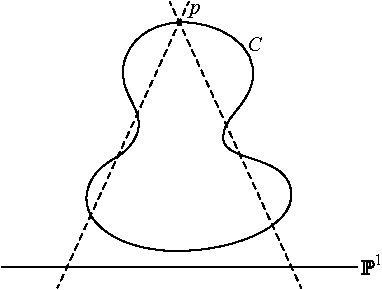
\includegraphics[height=1.7in,trim=0 0 15 0,clip]{main/Fig05-3}%
\llap{\raise12pt\hbox{$\ssty\PP^1$}}
 \caption{Expression of a plane quartic $C$ of genus 3 as a 3-sheeted
\index{3-sheeted cover}%
 cover of $\PP^1$ by projecting the canonical model from a point on it.}
\index{quartic curve!of genus 3}%
 \label{g13 on quartic}
\end{figure}

There are other representations of $C$ as the normalization of a plane
curve. By
Clifford's theorem
\index{Clifford's theorem}%
 $C$ has no $g^2_3$, and the canonical system
is the only $g^2_4$, but there are plenty of models as plane
quintic curves:
\index{quintic curve!models}%
by Proposition~\ref{very ample}, if $\sL$ is any invertible sheaf
of degree 5, the linear series $|\sL|$ will be a basepoint free $g^2_5$
as long as $L$ is not of the form $K+p$, so that $\phi_\sL$ maps $C$
birationally
onto a
plane quintic curve
\index{plane quintic}%
$C_0 \subset \PP^2` `$. These can
also be described geometrically in terms of the canonical model: any
such invertible sheaf $\sL$ is of the form $2K-p-q-r$ for some trio of
points $p, q, r \in C$ that are not collinear in the
canonical model,
\index{canonical model}%
and we see  that $C_0$ is obtained from the canonical model of $C$ by
applying a
Cremona transform
\index{Cremona transformation}%
with respect to the points $p, q$ and $r$,
that is, by applying the birational transformation
of the plane defined by the linear series of conics through $p,q,r$.

Proposition~\ref{very ample} implies that a divisor $D$ of degree 6 is
very ample if and only if it is not of the form $K+p+q$ for any $p, q
\in C$ and since the family of invertible sheaves on $C$ has dimension 3,
we see that a general invertible sheaf of degree 6 is very ample (indeed,
this is a simple case of Theorem~\ref{g+3 theorem}).

If $C\subset \PP^3$ is a curve of genus 3 embedded as a curve of degree
6, then $C$ cannot lie on a singular quadric since by
Example~\ref{Div of quadric} it would
have to be a complete intersection of the quadric with a cubic, and then
such a curve has genus 4. If $C$ lies on a smooth quadric
in class $(a,b)$ then $a$ or $b$ would be 2, so $C$ would be
hyperelliptic, and conversely any curve in class $(2,4)$
is a hyperelliptic curve of genus 3, degree 6.

Thus if $C$ is not hyperelliptic, then $C$ does not lie on a quadric
surface. We have $h^0(\sO_{\PP^3}(3)) = 20$ while, by the Riemann--Roch
formula, $h^0(\sO_C(3)) = 18-3+1= 16$, so $C$ lies on (at least) 4
independent cubics. Each of these cubics must be irreducible, so any
two of them
intersect in a curve of degree 9 containing $C$ and another component
or components $D$ of degree totaling 3. By
Bertini's theorem
\index{Bertini's theorem}%
if we choose two \emph{general} cubics containing $C$, then each of the
components of $D$ will be smooth. We shall see in
Theorem~\ref{liaison genus formula-first version}
that the arithmetic genus of $D$ must be 0;
thus $D$ must be a
twisted cubic
\index{twisted cubic}%
 curve. The ideal of the twisted cubic
is generated by the $2\times 2$ minors of a matrix of the form
$$
\begin{pmatrix}
 \ell_0& \ell_1&\ell_2\\
 \ell_1& \ell_2&\ell_3\\
\end{pmatrix}
$$
where the $\ell_i$ are linear forms,
and it follows that the two cubics can be written as the two $3\times 3$
minors involving the first two rows of  a matrix of the form
$$
\begin{pmatrix}
\label{hilbert-burch matrix}
 \ell_0& \ell_1&\ell_2\\
 \ell_1& \ell_2&\ell_3\\
\ell_4& \ell_5&\ell_6\\
 \ell_7& \ell_8&\ell_9\\
\end{pmatrix}
$$
where $\ell_4,\dots,\ell_9$ are linear forms as well.
From the
Hilbert--Burch theorem
\index{Hilbert--Burch theorem}%
(Corollary~\ref{Hilbert-Burch}) one can
show that the ideal of $C$ is generated by the four $3\times 3$ minors
of this matrix, whose columns generate
the
syzygies
\index{syzygy}%
of the ideal of the curve.

\section{Theta characteristics}

In this section we sketch the algebraic theory of theta characteristics,
\index{theta characteristic|(}%
starting with the case of curves of genus 3.

Suppose that $C \subset \PP^2$ is a smooth plane curve. A \emph{bitangent}
\index{bitangent}%
to $C$ is a line $L \subset \PP^2$ that is either tangent to $C$ at
two distinct points, or has contact of order $\geq 4$ with $C$ at a
point. Alternatively, we can say that a bitangent  corresponds to an
effective divisor of degree 2 on $C$ such that $2D$ is contained in the
intersection of $C$ with a line $L \subset \PP^2` `$.

A naive dimension count suggests that a smooth plane curve should have
a finite number of bitangents (it's one condition on a line $L \in
(\PP^2)^*$
to be tangent to $C$, so it should be two conditions for
it to be bitangent). Indeed, this is the case; by
B\'ezout's theorem
\index{Bezout@B\'ezout's theorem}%
a
conic or cubic curve cannot have any bitangents, but as we will show in
Section~\ref{plane curve pluecker} every smooth curve of degree $d \geq
4$ has
$$
12\,\mbinom{d+1}{4} - 4d(d-2),
$$
counted with appropriate multiplicities\emdash for example, a line simply
tangent to~$C$ at 3 points  counts as three bitangents. Accordingly,
\index{bitangent!to a plane quartic}%
\index{quartic curve!28 bitangents}%
a smooth plane quartic has 28 bitangents. (Figure~\ref{trott}
illustrates a special case in which all these bitangents
are realized over $\RR$.  The first explicit such example was published by
Pl\"ucker; see his drawing on page \pageref{fig28bitangents}.)

\begin{figure}
\centerline {\centerline{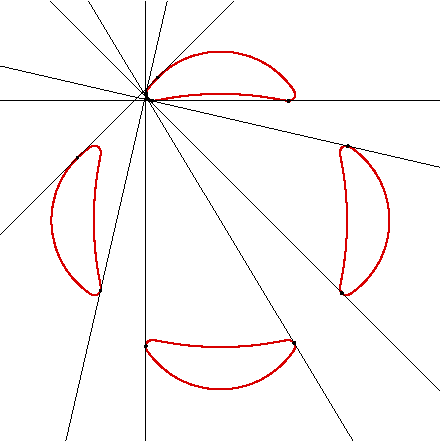
\includegraphics[height=2in]{main/Trott-cropped}}}
 \caption{The smooth plane quartic
$144 ( x^4 + y^4 ) - 225 ( x^2 + y^2 ) + 350 x^2 y^2 + 81 = 0$,
known as the Trott curve
\protect\citeyear{Trott}, has all 28 bitangents real.
\index{Trott quartic}%
(Only seven are shown for neatness. The involution $x \leftrightarrow -x$ gives
$7-1 =6$ more, then $y\leftrightarrow -y$ gives $13-2=11$ more, and
$x\leftrightarrow y$ the
remaining four.)}
\label{trott}
\end{figure}

The bitangents to a smooth plane quartic $C$ (a canonical curve of genus
3) have a special significance: since $4 = 2 \times 2$, if $D = p+q$ is
a bitangent, then the divisor $2D$ comprises the complete intersection
of $C$ with a line; in other words, we have a linear equivalence
$$
2D \sim K_C
$$
or equivalently the invertible sheaf $\cO_C(D)$ is a
square root of the canonical sheaf
\index{square root of canonical sheaf}%
\index{canonical sheaf!square root of}%
of $C$. Because of their appearance in the theory of
\index{theta function}%
theta functions,
Riemann
\index{Riemann @Riemann, Georg Friedrich Bernhard}%
named the square roots of the canonical sheaf
\emph{theta characteristics}.

How many such square roots are there? If $\cL$ and $\cM$ are invertible
sheaves with $\cL^2 = \cM^2 = K$, then $\cL$ and $\cM$ differ by an
invertible sheaf of order 2:
$$
\cM = \cL \otimes \cF, \quad \text{where} \quad \cF \otimes \cF \sim
\cO_C.
$$
In other words, $\cF$ is an invertible sheaf of degree 0 and, having
fixed $\sL$,  the other sheaf, $\cM$, corresponds to a point of order
2 in the
Picard group
\index{Picard group}%
$\Pic_0(C)$. Since we've seen that $\Pic_0(C) =
\Jac(C)$ is a complex torus of dimension
$g =\nobreak 3$\emdash the quotient of $\CC^3$
by a lattice $\Lambda \cong \ZZ^6$\emdash we see that there are $2^6 = 64$
such invertible sheaves, and thus, given that there is some invertible
sheaf $\cL$ satisfying $\cL^2 \cong K_C$, there are exactly $64 = 2^{2g}$
of them.

The reader will have noticed that the number 64 of theta characteristics
does not agree with the number 28 of bitangents. The reason is
that
bitangents correspond to \emph{effective} divisors $D$ with $2D
\sim K$, while a theta characteristic $\cL$ may have $h^0(\cL) = 0$,
that is, may not correspond to an effective divisor.
This situation also occurs in other genera.
What can we say about the dimensions $h^0(\cL)$ of the space of sections
of the theta characteristics on $C$?

 There is a beautiful partial answer to this question, which can be
 deduced from a remarkable fact: the dimension $h^0(\cL)$ of the space
 of sections of a theta characteristic mod 2 is invariant in families.
We will now
sketch the necessary results; see \cite{MumfordPaper} and \cite{JHPaper}
for a full treatment.

 \begin{theorem}
 \label{locally constant sign}
 Let $\cC \to B$ be a family of smooth curves, and $\cL_b$ a family of
 theta characteristics on the curves in this family\emdash in other words, an
 invertible sheaf $\cL$ on $\cC$ such that $(\cL|_{C_b})^2 \cong K_{C_b}$
 for each $b \in B$.
If
$f : B \to \ZZ/2$
is defined by
 $$
 f(b) = h^0(\cL|_{C_b}) \;  \; (\mathrm{mod\ } 2),
 $$
then $f$ is locally constant.
\unif
\end{theorem}

We say that a theta characteristic $\cL$ is \emph{even} or \emph{odd}
\index{theta characteristic}%
according to the parity of $h^0(\cL)$. Given the irreducibility of the
space of smooth irreducible curves of genus $g$ (which we'll discuss
in Chapter~\ref{CurvesModuliChapter}),
Theorem~\ref{locally constant sign}
suggests that all curves of genus $g$ have the same number of
even (equivalently, of odd) theta characteristics, and this is in fact
the case.

\begin{theorem}
\label{number of theta characteristics}
If $C$ is a curve of genus $g$, then of the $2^{2g}$ theta characteristics
\index{theta characteristic!number of --s}%
on $C$ there are $2^{g-1}(2^g + 1)$ even theta characteristics and
$2^{g-1}(2^g-1)$ odd theta characteristics.
\unif
\end{theorem}

Using Theorem ~\ref{locally constant sign} and the connectedness of the
moduli space of curves,
Theorem~\ref{number of theta characteristics} is reduced to the case when
$C$ is hyperelliptic. We will
compute the number of theta characteristics in the hyperelliptic case
later in this section (page~\pageref{theta characteristic count}).

For
a nonhyperelliptic curve $C$ of genus 3, the
dimension $h^0(\cL)$ of a theta characteristic $\cL$ cannot be $\geq 2$, so
the odd theta characteristics are exactly the effective theta
characteristics, and  this says
that there are $2^{g-1}(2^g-1)
= 28$ effective theta characteristics corresponding to the 28 bitangents.
\index{bitangent!to a plane quartic}%


We will present  a proof of Theorem~\ref{locally constant sign} using
an ingenious construction of
\index{genus 3 curve|)}%
Mumford's,
\index{Mumford @Mumford, David}%
after explaining the necessary facts about
quadratic forms
\index{quadratic form}%
in an even
number of variables.
\smallbreak

\begin{fact}
\label{isotropic facts}
Suppose that $V$ is a $2n$-dimensional complex vector space with a
nondegenerate
bilinear form
\index{bilinear form}%
$Q$. An
\emph{isotropic subspace} for $Q$ is a subspace $\Lambda \subset V$ such that
\index{isotropic subspace}%
$Q(\Lambda, \Lambda) = 0$.

 \begin{enumerate}
\item The maximal isotropic subspaces for $Q$ have dimension $n$.

\item The set of maximal isotropic subspaces for $Q$ is a subvariety of
the
Grassmannian
\index{Grassmannian}%
$G(n,V)$, of dimension $\tbinom{n}{2}$, that has exactly
two connected components.

\item If $\Lambda, \Lambda' \subset V$ are any two maximal isotropic
subspaces, then
$$
\let\quad\enspace
\null\hskip\leftmargini
\dim(\Lambda \cap \Lambda') \equiv n \text{ (mod 2)} \quad \iff \quad
\Lambda, \Lambda' \text{ \,belong to the same ruling.}
$$
\end{enumerate}

A  proof is given in \cite[pp.~735--740]{Griffiths-Harris1978}.
\end{fact}

\begin{remark}
The first assertion in
Cheerful Fact \ref{isotropic facts}
is
elementary: since the map
$\widetilde Q : V \ruto \cong V^*$ associated to the form $Q$ carries
\index{isotropic subspace}%
an isotropic subspace to its annihilator, there can't be an isotropic
subspace of dimension $>n$; and similarly if $\Lambda \subset V$ is any
isotropic subspace of dimension $<n$ we can include $\Lambda$ in a larger
isotropic subspace by adding any vector $v$ with $\overkern20 Q(v,v) = 0$
for the induced bilinear form $\overkern20 Q$ on $\ann(\Lambda)/\Lambda$.

The second and third assertions are less elementary, but the reader may
already have seen the first two nontrivial cases of each:
\end{remark}

\begin{example}
When $n=2$ the form $Q$ corresponds to a smooth quadric surface
in $\PP^3` `$, and the lines on this surface correspond to the isotropic
2-planes in $\CC^4` `$. There are two rulings by lines, and lines of
opposite rulings meet in a point, while lines of the same ruling are
either disjoint or equal.
\end{example}

\begin{example}
When $n=3$, the Grassmannian $\GG(1,3)$, in its
Pl\"ucker embedding,
\index{Pl\"ucker embedding}%
\index{Grassmannian}%
\index{G@$\GG(1,3)$}%
is a smooth quadric in $\PP^5` `$. The isotropic subspaces in the two distinct
components are easy to describe: in one component they are the projective
2-plane of lines containing a given point $p \in \PP^3` `$. In the other
component they are  the planes corresponding to the lines contained in a
given plane $H \subset \PP^3` `$. These families visibly satisfy property (3) above.
See Exercise~\ref{G13}.
\end{example}

\begin{proof}[Proof of Theorem~\ref{locally constant sign}] Suppose that $C$ is a smooth curve of genus $g$, and
let $\cL$ be
an invertible sheaf on $C$ with $\cL^2 \cong K_C$\emdash that is, a theta
characteristic. Choose a divisor $D = p_1 + \dots + p_n$ of degree $n>
g-1$ consisting of distinct points, and let $V$ be the $2n$-dimensional
vector space
$$
V \colonequals  H^0( \cL(D) / \cL(-D) ).
$$
From the exact sequence
$$
0\to \cL(-D) \to \cL(D) \to \cL(D)/\cL(-D) \to 0
$$
we see that
the sheaf $ \cL(D) / \cL(-D)$ is supported on $D$, with stalk
isomorphic to $\cO_p/\gm_{C,p}^2$ of dimension 2 at each $p \in D$. We
can define a bilinear form on $V$ by setting
\index{residue}%
$$
Q(\sigma, \tau) \colonequals  \sum_i \Res_{p_i}(\sigma \tau)
\vspace*{-3pt}
$$
where we use the isomorphism $\cL^2 \cong K_C$ to identify the product
$\sigma\tau$ with a rational differential.

We now introduce two isotropic subspaces for $Q$.
The first is
$$
\Lambda \colonequals  H^0( \cL / \cL(-D) ),
$$
which
is isotropic because the product
of two of its elements
corresponds to a regular differential, and so has no residues.
Second, we set
$$
\Lambda' \colonequals  \im\left( H^0(\cL(D)) \to H^0( \cL(D) / \cL(-D) ) \right)
.
$$
Since  $H^0(\cL(-D)) = 0$, the map is injective and according to
the Riemann--Roch theorem we have
$h^0(\cL(D)) = n$, so this is again an $n$-dimensional
subspace of~$V$; it's isotropic because the sum of the residues of a
global rational differential on $C$ is 0. Finally,
$$
H^0(\cL) \cong \Lambda \cap \Lambda',
$$
and Theorem~\ref{locally constant sign} follows.
\end{proof}




\subsection*{Counting theta characteristics (proof of Theorem~\ref{number of theta characteristics})}

One
way to count the number of odd and even theta characteristics on
\label{theta characteristic count} % used for page number
a curve of genus $g$ is  to describe
them
explicitly in the case of
a hyperelliptic curve and
use Theorem~\ref{locally constant sign}
to deduce the corresponding statements for any smooth curve of genus~$g$.
The reader
may wish to
try a relatively simple case in
Exercise~\ref{theta char on genus 2} before looking at the general
case below.
We start with some preliminary calculations:

\begin{lemma}
\label{summing binomials}
For any positive integer $n$,
we have
\let\binom\mbinom
\begin{gather}
\let\;\relax
\sum_{k=0}^n \binom{2n}{2k} \; = \; \sum_{k=0}^{n-1} \binom{2n}{2k+1}
\; = \; 2^{2n-1}
,\\
\sum_{k=0}^n \binom{4n}{4k} = 2^{4n-2}  + (-1)^n 2^{2n-1},
\quad \sum_{k=0}^{n-1} \binom{4n}{4k+2} = 2^{4n-2} - (-1)^n  2^{2n-1}
,\\
\sum_{k=0}^n \binom{4n+2}{4k+1} = 2^{4n} + (-1)^n 2^{2n},
\quad \sum_{k=0}^{n-1} \binom{4n}{4k+3} = 2^{4n} - (-1)^n  2^{2n}
.
\end{gather}
\end{lemma}

\begin{proof}
\let\binom\mbinom
Equality (1) is
elementary; by the binomial theorem, we have
$$
2^{2n} = (1+1)^{2n} = \sum_{l = 0}^{2n}@\binom{2n}{l} \quad \text{and}
\quad 0 = (1-1)^{2n} = \sum_{l = 0}^{2n}@(-1)^l\binom{2n}{l}
,
$$
and taking the sum and the difference of these two equations yields the
result.

The equalities in (2) follow
similarly by applying the binomial theorem to the
expression $(1 + i)^{4n} = (-1)^n2^{2n}$. Equating the real parts, we have
$$
\sum_{k=0}^n \binom{4n}{4k} - \sum_{k=0}^{n-1} \binom{4n}{4k+2} =
(-1)^n2^{2n}
,
$$
while by
(1)
we have
$$
\sum_{k=0}^n \binom{4n}{4k} + \sum_{k=0}^{n-1} \binom{4n}{4k+2} =
2^{4n-1}.
$$
Taking the sum and difference of these equations yields the desired
formulas.

For (3)
we apply the binomial theorem to the expression $(1 + i)^{4n+2} =
 (-1)^n2^{2n+1}i$. Equating the imaginary parts, this gives
\let\;\relax
$$
\sum_{k=0}^n \binom{4n+2}{4k+1} - \sum_{k=0}^{n-1} \binom{4n+2}{4k+3}
\; = \; (-1)^n2^{2n+1}
,
$$
whereas by
(1),
$$
\sum_{k=0}^n \binom{4n+2}{4k+1} + \sum_{k=0}^{n-1} \binom{4n+2}{4k+3}
\; = \; (-1)^n 2^{4n+1}
,
$$
and as before taking the sum and difference
yields the
result.
\end{proof}

We will count the number of theta characteristics on a hyperelliptic
curve in terms of sums of subsets of the ramification points, so we need
to know what linear equivalences exist among sums of these subsets:

\begin{lemma}
\label{ramification point relations}
Let $C$ be the hyperelliptic curve of genus $g$ expressed as a 2-sheeted
cover of $\PP^1$ with ramification points $p_1,\dots,p_{2g+2}$. The
divisor class of
 any half of the ramification points is equal to the divisor class of
 the other half, but there are no
 smaller relations. More precisely,
 let $I_1,I_2$ be subsets of $\{1,\dots 2g+2\}$
and set
$$
D_i = \sum_{j\in I_i} p_j.
$$
The divisors $D_1,D_2$ are linearly equivalent if and only if $I_1 `= I_2$
or they
have the same cardinality $g+1$ and $I_1`\cup I_2 = \{1,\dots, 2g+2\}$.
\end{lemma}

\begin{proof}
The ``if'' part is simply
Corollary~\ref{relation on ramification points} above.

For the ``only if'' part, subtracting whatever points $D_1$ and $D_2$
have in common we may suppose
that $I_1`\cap I_2 = \emptyset$. If $D_1\sim D_2$, it follows at once that
they have the same degree, $d\leq g+1$, and we must show that either $d=0$
or $d=g+1$.

We have $D_1\sim D_2$
if and only if
$D_1+D_2\equiv 2D_1$. If
$d\leq g$ we have $r(2D_1) = d$: for $d<g$ this is
the extremal case of
Clifford's theorem,
\index{Clifford's theorem}%
while for $d = g$ this follows
simply from the
Riemann--Roch formula.
\index{Riemann--Roch formula}%
Thus in case $d \leq g$ every divisor in $|2D_1|$
is a sum of $d$ fibers of the
2 to 1 map of $C$ to $\PP^1` `$, and for such a divisor to be a sum of
distinct points $p_i$
the degree $d$ must be 0, concluding the argument.
\end{proof}

Returning
now
to the counting, let $C$ be the hyperelliptic curve of genus
$g$, \null
expressed as a 2-sheeted cover of $\PP^1` `$, with ramification points
$p_1,\dots,p_{2g+2}$.

First of all, if we denote the class of the unique $g^1_2$ on $C$ by
$E$, and $D$ is any theta characteristic, then $D+E$ will be effective,
and so we can write
$$
D \sim mE + F
$$
with $-1 \leq m \leq (g@{-}@1)/2$ and $F$ the sum of $g-1-2m$ distinct
points $p_i$.
This representation is unique unless
$m=-1$; in that case, we note that the sum of $g+1$ of the branch
points of $C$ is linearly equivalent to the sum of the other $g+1$ by
Corollary~\ref{relation on ramification points}. Thus the total number of
theta characteristics is a sum of binomial coefficients; if $g$ is odd,
it is
$$
\let\binom\mbinom
\binom{2g+2}{0} + \binom{2g+2}{2} + \binom{2g+2}{4} + \dots +
\binom{2g+2}{g-1} + \frac{1}{2}\binom{2g+2}{g+1}
$$
and similarly if $g$ is even it is
$$
\let\binom\mbinom
\binom{2g+2}{1} + \binom{2g+2}{3} + \binom{2g+2}{5} + \dots +
\binom{2g+2}{g-1} + \frac{1}{2}\binom{2g+2}{g+1}.
$$
In either case, we are adding up every other entry in the $(2g+2)$-nd
row of Pascal's triangle, starting from the left and ending up with one
half of the middle term. This sum is exactly one half of the sum of every
other entry in the whole row; by the first part of
Lemma~\ref{summing binomials}
this
equals
$\sfrac{1}{4} \cdot 2^{2g+2} = 2^{2g}$.

Finally, we can add up the number of even and odd theta characteristics
separately simply by taking every other term in the sums above;
using
equalities (2) and (3) in
Lemma~\ref{summing binomials}
(in case $g$ is odd and even, respectively) we can conclude that $C$
has $2^{g-1}(2^g-1)$ odd theta characteristics and $2^{g-1}(2^g+1)$
even theta characteristics. By Theorem~\ref{locally constant sign} and
the connectedness of the space of smooth irreducible curves of genus
$g$, this count then holds for all curves of genus $g$, establishing
Theorem~\ref{number of theta characteristics}.
\qed

 It is also
 possible to describe the configurations of odd and even theta
characteristics as subsets of the set $S$ of all theta characteristics,
which as we've seen is a principal
homogeneous space for the group
$\Jac(C)_2 \cong (\ZZ/2\ZZ)^{2g}$ of
points of order 2 on the Jacobian.
\index{Jacobian!points of order 2}%
 This leads to an alternative proof of
Theorem~\ref{number of theta characteristics} as in \cite{JHPaper}.

\begin{fact}
There is more to say about the configuration of theta characteristics.
As noted, if we choose any theta characteristic on a curve $C$, we may
 identify the set $S^-$ of odd theta characteristics with a subset of the
 group $\Jac(C)_2$ of points of order 2 on the Jacobian of $C$. We might
 expect that some 4-tuples of these points will add up to 0 in $\Jac(C)$;
 in other words, there should exist some 4-tuples $\cL_1,\dots,\cL_4
 \in S^-$ such that
$$
\cL_1\otimes \dots \otimes\cL_4 = 2K_C.
$$
What this means in the case of genus $g=3$ is that among the 28 bitangents
\index{bitangent!to a plane quartic}%
to a smooth plane quartic curve $C$, there are some subsets of 4 whose
eight points of tangency form the intersection of $C$ with a plane
conic. From the more detailed knowledge of the configuration $S^-$
we can say how many. Indeed, the number was first found by Salmon
\index{Salmon @Salmon, George}%
\citeyear{MR0115124};
it is 315.
\index{theta characteristic|)}%
\end{fact}

\section{Exercises}
 \begin{exercise}
  We have seen that a curve $C$ of genus $g=1$ is expressible as a
  2-sheeted cover of $\PP^1$ branched over four points; that is, as
  the smooth projective curve associated to the affine curve $C^\circ
  \subset \AA^2$ given by $y^2 -
\smash{\prod_{i=1}^{\smash{\lower1.5pt\hbox{$\ssty4$}}} (x-\lambda_i)}$.
  Show that
  the closure $\overkern22{C^\circ}$ of $C^\circ \subset \AA^2$ in either
  $\PP^2$ or $\PP^1 \times \PP^1$ consists of the union of $C^\circ$ with
  one additional point, with that point a tacnode of $\overkern22{C^\circ}$
  in either case.
  \tohint{6.1}
  \end{exercise}

\begin{exercise}
Find the number of
3-sheeted covers
\index{3-sheeted cover}%
$C \to \PP^1$ of genus $g$ with
simple branching except for one point of
\index{simple branch point}%
\index{branch point!simple}%
total ramification
\index{total ramification}%
(that is,
one point with just a single preimage point.)
\tohint{6.1}
\end{exercise}

\begin{exercise}
Let $C$ be a curve of genus $g$. How many
unramified double covers
of $C$
\index{2-sheeted cover!unramified}%
are there?
\tohint{6.3}
\end{exercise}

\begin{exercise}
Show that unramified
double covers
of a smooth curve $C$ are in one-to-one
correspondence
with invertible sheaves $\sL$ on $C$ such that $\sL^2 \cong \sO_C$,
that is with the
2-torsion points
\index{Jacobian!points of order 2}%
of $\Jac(C)$.
\tohint{6.4}
\end{exercise}

\begin{exercise} Let $E$ be a curve of genus 1, and $q_1,\dots,q_b \in
E$. How many double covers $C \to E$ are there branched over the $q_i$?
\tohint{6.5}
\end{exercise}

\begin{exercise}
\label{ideal of genus 2 degree 5}
In
this
exercise, we ask you to complete the
earlier
description
of the ideal of a quintic space curve of
genus 2,
keeping the notation of page~\pageref{genus 2 quintic}.

Show that for any pair of lines $L, L'$ of the appropriate ruling of $Q$,
\index{quintic curve!of genus 2}%
the three polynomials $Q$, $S_L$ and $S_{L'}$ generate the homogeneous
ideal $I(C)$. Find relations among them. Write out the minimal resolution
of $I(C)$.
\tohint{6.6}
\end{exercise}

\begin{exercise}
% an easy case the reader can do before reading the general treatment.
\label{theta char on genus 2}
 Let $C$ be a curve of genus 2, expressed as a 2-sheeted cover of $\PP^1$
 with ramification points $p_1,\dots,p_6$. In this exercise we will
 count the number of
 even and odd theta characteristics.
The text contains the count for a hyperelliptic curve of any genus;
we offer
the case of genus 2 as a warmup.
 \begin{enumerate}
 \item Show that the theta characteristics on $C$ are either of the
 form $\cL = \cO_C(p_i)$ or of the form $\cL = \cO_C(p_i + p_j - p_k)$
 with $i, j, k$ distinct.
 \item Show that in the first case we have $h^0(\cL) = 1$, and in the
 second case we have $h^0(\cL) = 0$.
 \item Finally, show that there are six of the former kind, and 10 of
 the latter, making $2^4 = 16$ in all.
 \tohin{6.7}
 \end{enumerate}\label{tnih6.7}
 \end{exercise}

\begin{exercise}
\label{nodal quartic}
Let $C$ be a  curve of genus 2 and let $\sL\in \Pic_4(C)$ be an invertible
sheaf of the form $\sL = K_C(p+q)$ with $p \neq q$ and $p+q \not\sim K_C$
as in~\ref{p+q not g12}. Show that
\begin{enumerate}
\item $h^0(\sL(-2r))= 1$ for any point $r \in C$, and
\item $h^0(\sL(-2p-2q)) = 0$.
\end{enumerate}
Deduce from this that the map $\phi_\sL$ is an immersion, and that the
tangent lines to the two branches of $\phi_\sL(C)$ at the point $\phi_\sL(p)
= \phi_\sL(q)$ are distinct, meaning the point $\phi_\sL(p) = \phi_\sL(q)$
is a node of $\phi_\sL(C)$.
\tohint{6.8}
\end{exercise}

\begin{exercise}
\label{G13}
We can represent any line in $\PP^3$ as the row space of a $2\times 4$ matrix by choosing
\index{G@$\GG(1,3)$}%
 2 points on the line and
using their
coordinates as the rows. The \emph{Pl\"ucker coordinates} of the line are
\index{Pl\"ucker coordinates}%
the six $2\times 2$ minors
$$
\{p_{i,j}\}_{0\leq i<j\leq 3}
$$
of this matrix. They are independent, up to a common scalar multiple,
of the two points chosen, and define the \emph{Pl\"ucker embedding}
\index{Pl\"ucker embedding}%
of the
Grassmannian
\index{Grassmannian}%
$\GG(1,3)$ in $\PP^5` `$.

The minors $p_{i,j}$  satisfy a nonsingular quadratic equation: if we
stack two copies of the $2\times 2$
matrix to produce a $4\times 4$ matrix, its determinant is zero, and
the Laplace expansion of this determinant
is the \emph{Pl\"ucker equation}
\index{Pl\"ucker equation}%
$$
p_{0,1}p_{2,3}-p_{0,2}p_{1,3}+p_{0,3}p_{1,2} = 0.
$$

\begin{enumerate}
\item Show that the quadratic form
$
Q = p_{0,1}p_{2,3}-p_{0,2}p_{1,3}+p_{0,3}p_{1,2}
$
is non\-singular, and deduce that it generates the ideal of $\GG(1,3)$
in $\PP^5` `$.
\item
Write the bilinear form corresponding to $Q$ as the determinant of a
matrix, and deduce that
two points in $\GG(1,3)$ correspond to vectors that pair to 0 if and
only if they correspond to lines that intersect.
\item Deduce that a maximal isotropic subspace for $Q$ corresponds either to
the set of lines containing a given point or the set of lines contained
in a given plane; and that two such sets of lines
of the same type
meet in a single point or coincide.
\end{enumerate}
\end{exercise}

